\documentclass[prb,9pt,notitlepage]{revtex4-1}
%\documentclass[a4paper,twocolumn,9pt]{article}

%\usepackage{geometry}
%\geometry{a4paper,top=2.5cm,bottom=2cm,inner=1.5cm,outer=1.5cm}

\usepackage{mwe}% just for the example content
\usepackage{color}
\usepackage{latexsym,amsmath}
\usepackage{physics}
\usepackage{listings}
\usepackage[dvipsnames]{xcolor}
\usepackage{parskip}
\usepackage{hyperref}
%\usepackage{dblfloatfix}
%\usepackage{subfig}
\definecolor{linkcolor}{rgb}{0,0,0.65}%hyperlink
\definecolor{shadecolor}{rgb}{0.93, 0.93, 0.93}
%\usepackage[pdftex,colorlinks=true, pdfstartview=FitV, linkcolor= linkcolor, citecolor= linkcolor, urlcolor= linkcolor, hyperindex=true,hyperfigures=true]{hyperref} %hyperlink%
%\usepackage[backend=biber, sorting=ynt]{biblatex}
%\usepackage{ragged2e} % to justify caption
%\addbibresource{bibliography.bib}
 \usepackage{booktabs}

\usepackage[T1]{fontenc}
\usepackage{xcolor}
\usepackage{lmodern}
\usepackage{listings}
\lstset{language=[95]Fortran,
  backgroundcolor=\color{shadecolor},
  basicstyle=\ttfamily,
  keywordstyle=\color{blue},
  commentstyle=\color{gray},
  stringstyle=\color{red},
  showstringspaces=false
  %morecomment=[l]{!\ }% Comment only with space after !
}

\usepackage{tabularx}

\usepackage{fancyhdr}
\pagestyle{fancyplain}% <- use fancyplain instead fancy
\fancyhf{}
\fancyhead[R]{\today}
\fancyhead[L]{Alessandro Lambertini}
\fancyfoot[L]{Quantum information and computing}
\fancyfoot[C]{Report 2}
\fancyfoot[R]{\thepage}

\renewcommand{\headrulewidth}{0pt}

\usepackage{float}
\usepackage{siunitx}




\begin{document}
\title{Quantum information and computing: Exercises report, week 4. \\ Multi-run script \& Automated fits }

\author{Alessandro Lambertini}


\date{\today}

\begin{abstract}
Through the exercise of this week, we try to numerically solve a physical problem for the first time. We describe the 1-D quantum harmonic oscillator by solving the eigenvalues problem exploiting the subroutines written for the previous exercises. In particular, we are requested to compute the first k eigenvalues and the first k eigenstates of the oscillator.
\end{abstract}

\maketitle

\section{Theory}
We consider the 1-D quantum harmonic oscillator defined by the Hamiltonian and the correspondent time-independent Schroedinger equation:
\begin{equation}
  H = \frac{\hat{p}^2}{2m} + \frac{1}{2} m\omega^2\hat{q}^2 \quad \longrightarrow \quad \left[-\frac{\hbar^2}{2m}\frac{d^2}{d^2x} + \frac{1}{2}m \omega^2x^2\right]\psi(x) = E \psi(x)
\end{equation}
The solutions of this eigenvalues problem have a closed and recursive form, which is:
\begin{equation}
  E_n = (n+\frac{1}{2} )\hbar\omega \qquad   \psi_{n}(x)={\sqrt {\frac {1}{2^{n}n!}}}\left({\frac {m\omega }{\hbar \,\pi }}\right)^{1/4}H_{n}\left({\sqrt {\frac {m\omega }{\hbar }}}x\right)e^{-{\frac {mx^{2}\omega }{2\hbar }}}
\end{equation}
Where $H_n$ are the Hermite polynomials.

To solve numerically this equation by means of the finite difference method we introduce a discretization of our space with a constant spacing $h$.
At second order in h the second derivative of $\psi(x)$ at $x_n$ can be approximated by:
\begin{equation}
  \psi''_n = \frac{\psi_{n+1}-2\psi_n+\psi_{n-1}}{h^2} + \mathcal{O}(h^2)
\end{equation}
Therefore, we have a discretization of our problem given by:
\begin{equation}
\frac{1}{h^2}\left( \begin{array}{cccccccc} \frac{2\hbar^2}{2m} + V_1 & -1 & 0 & \cdots & 0 & 0 & 0  \\ -1 & \frac{2\hbar^2}{2m}+ V_2 & -1 & \cdots & 0 & 0 & 0  \\ & & &\vdots  \\ 0 & 0 & 0 & \cdots&-1 & \frac{2\hbar^2}{2m}+ V_{N-1} &-1& \\ 0 & 0 & 0 & \cdots&0 &-1& \frac{2\hbar^2}{2m}+ V_{N-1} \\ \end{array}
\right)\ket{\psi} = E\ket{\psi}
\end{equation}
where $V_i=V(x_i)$.
\section{Code development}
In order to accomplish the task of solving the eigenvalue problem above mentioned i essentially exploited the subroutine written for the last exercise. However, before diagonalizing the matrix, it must be initialized. For this purpose, I wrote a subroutine to do it in the proper way:

\begin{lstlisting}
subroutine init_tridiag_qao_matrix(matrix, x_max,xx, N, freq, mass, h_bar)
  complex(kind=8), dimension(:,:), allocatable :: matrix
  real(kind=8), dimension(:), allocatable :: xx
  real(kind=8) :: Re_z, x_max,step,freq,mass,h_bar
  integer(kind=8) ::  ii, N

  allocate(xx(N))
  allocate(matrix(N,N))

  step = 2*x_max/real(N-1,8)

  do ii=1,N
    xx(ii) = -x_max+(ii-1)*step
  end do

  !initialize the diagonal
  do ii=1,N
    Re_z = ((2*h_bar**2)/(2*mass) + (mass/2)*freq**2*xx(ii)**2*step**2)/step**2
    matrix(ii,ii) = cmplx(Re_z,0)
  end do

  Re_z = (-h_bar**2/(2*mass)/step**2)

  !initialize the lower elements
  do ii =1,N-1
    matrix(ii,ii+1) = cmplx(Re_z,0)
  end do

  !initialize the upper elements
  do ii = 2,N
    matrix(ii,ii-1) = cmplx(Re_z,0)
  end do

end subroutine init_tridiag_qao_matrix
!!!!!!!!!!!!!!!!!!!!!!!!!!!!!!!!!!!!!!!!!!!!!!!!!!!!!!!!!!!!!!!!!!!!!!!!
\end{lstlisting}
I decided to initialize both the upper half and the lower part of the matrix in order to make the subroutine more flexible, in the sense that in this way we do not have to care which half of the matrix is initialized when we use a \textit{laPACK} subroutine to diagonalize it. Moreover, the discretization of the space is built to be simmetric with respect to the origin.

Then, I wrote other two subroutines in order to print and store intermediate and final results:
\begin{lstlisting}
!!!!!!!!!!! write the first k entries of a real array in a file !!!!!!!!!!!
subroutine first_k_entries_on_file(title,vec,kk)
  character(len=*) title
  real(kind=8), dimension(:) :: vec
  integer(kind=8) :: ii, kk

  if ( kk .le. size(vec) ) then

    open(1,file=title,Access = 'append')
    do ii=1,kk
      write(1,'(I0,A,F0.15)') (ii-1),',',vec(ii)
    end do
    close(1)
  else
    !error handling
    write(*,*) 'size(vec) > k'

  end if
end subroutine first_k_entries_on_file
!!!!!!!!!!!!!!!!!!!!!!!!!!!!!!!!!!!!!!!!!!!!!!!!!!!!!!!!!!!!!!!!!!
\end{lstlisting}
With this subroutine one can store the first k entries of a real array in a file named \textit{title}, a check of the size of the array with respect to k is present.


With this subroutine instead we can write on file the first k columns of a real matrix and up to two vectors as the first and second columns of the file:
\begin{lstlisting}
subroutine vec_and_col_on_file(title,mm,kk,vec_1,vec_2)
character(len=*) title
real(kind=8), optional, dimension(:) :: vec_1,vec_2
real(kind=8), dimension(:,:) :: mm
integer(kind=8) :: ii, jj, kk

!both vec_1 and vec_2 are present and written as 1st and 2nd columns
if ( present(vec_2) .and. present(vec_1) ) then

  if ( (size(vec_2) .eq. size(vec_1) ) .and. &
  (size(vec_2) .eq. size(mm, dim=1) )) then

    open(1,file=title,Access = 'append')
    do ii=1,size(vec_1)
      write(1,*) vec_1(ii), ',', vec_2(ii), ',', (mm(ii,jj),',',jj = 1, kk)
    end do
    close(1)


  else
    !error handling
    write(*,*) 'size mismatch'

  end if

!only vec_1 is present and written as 1st column
elseif( present(vec_1) ) then
  if ( size(vec_1) .eq. size(mm, dim=1)) then

    open(1,file=title,Access = 'append')
    do ii=1,size(vec_1)
      write(1,*) vec_1(ii),',', (mm(ii,jj),',',jj = 1, kk)
    end do
    close(1)

  else
    !error handling
    write(*,*) 'size mismatch'
  end if

!only the matrix is present and the first k columns are written
else

  open(1,file=title,Access = 'append')
  do ii=1,size(vec_1)
    write(1,*) (mm(ii,jj),',',jj = 1, kk)
  end do
  close(1)
end if

end subroutine vec_and_col_on_file
\end{lstlisting}
These three subroutines and the ones used to test the program during its construction are collected and ready to be used in a module named \textit{ex06module} in a file named \textit{ex\_06\_module.f90}

With these three subroutine, in addition to the one to diagonalize the matrix, one can structure the program to complete the task of computing and storing the first k eigenvalues and eigenstates of the 1-D quantum harmonic oscillator. I choose to use natural units and set the parameters of the problem accordingly.
\begin{lstlisting}
program q_harm_osc
  use ex06module
  implicit none

  complex(kind=8), dimension(:,:), allocatable :: matrix
  real(kind=8), dimension(:), allocatable :: xx
  real(kind=8) :: Re_z, x_max,step,freq,mass,h_bar
  integer(kind=8) ::  ii, N, k_columns, k_entries
  double precision, dimension(:), allocatable :: eigv

  !set the parameters of the problem
  N=1000
  x_max = 10
  freq = 1
  mass = 0.5
  h_bar = 1
  step = 2*x_max/real(N-1,8)
  k_columns = 3
  k_entries = 100
  !initialize the matrix and store it in a file
  call init_tridiag_qao_matrix(matrix, x_max,xx, N, freq, mass, h_bar)
  call vec_and_col_on_file('original_matrix.txt',real(matrix), N, xx)
  !call write_a_vector('x',xx)

  !diagonalize and normalize the matrix
  call diag_hermit_matrix(matrix,eigv)
  matrix = matrix/sqrt(step)


  !store the first k eigenfunctions and the first k eigenvalues in a file
  call vec_and_col_on_file('x_and_columns.txt',real(matrix), k_columns, xx)
  call first_k_entries_on_file('first_k_eigenvalues.txt', eigv, k_entries)
end program q_harm_osc

\end{lstlisting}
In the program I initialize and store the matrix in a file named \textit{original\_matrix.txt}, then we diagonalize it and store the first k columns of the diagonalized matrix and the lattice array in a file called \textit{x\_and\_columns.txt}; finally I store the first k entries of the eigenvalue array in a file called \textit{first\_k\_eigenvalues.txt}.

\section{Results}
Here I show the comparison between the first three eigenfunctions computed with the program and the theorical ones, to do it I exploited a little gnuplot script. Moreover, a comparison between the first 110 eigenvalues computed and the theorical ones is presented. To set the parameters in the program, the interval and the step of the discretization, several attempts with different values have been made.
\begin{center}
    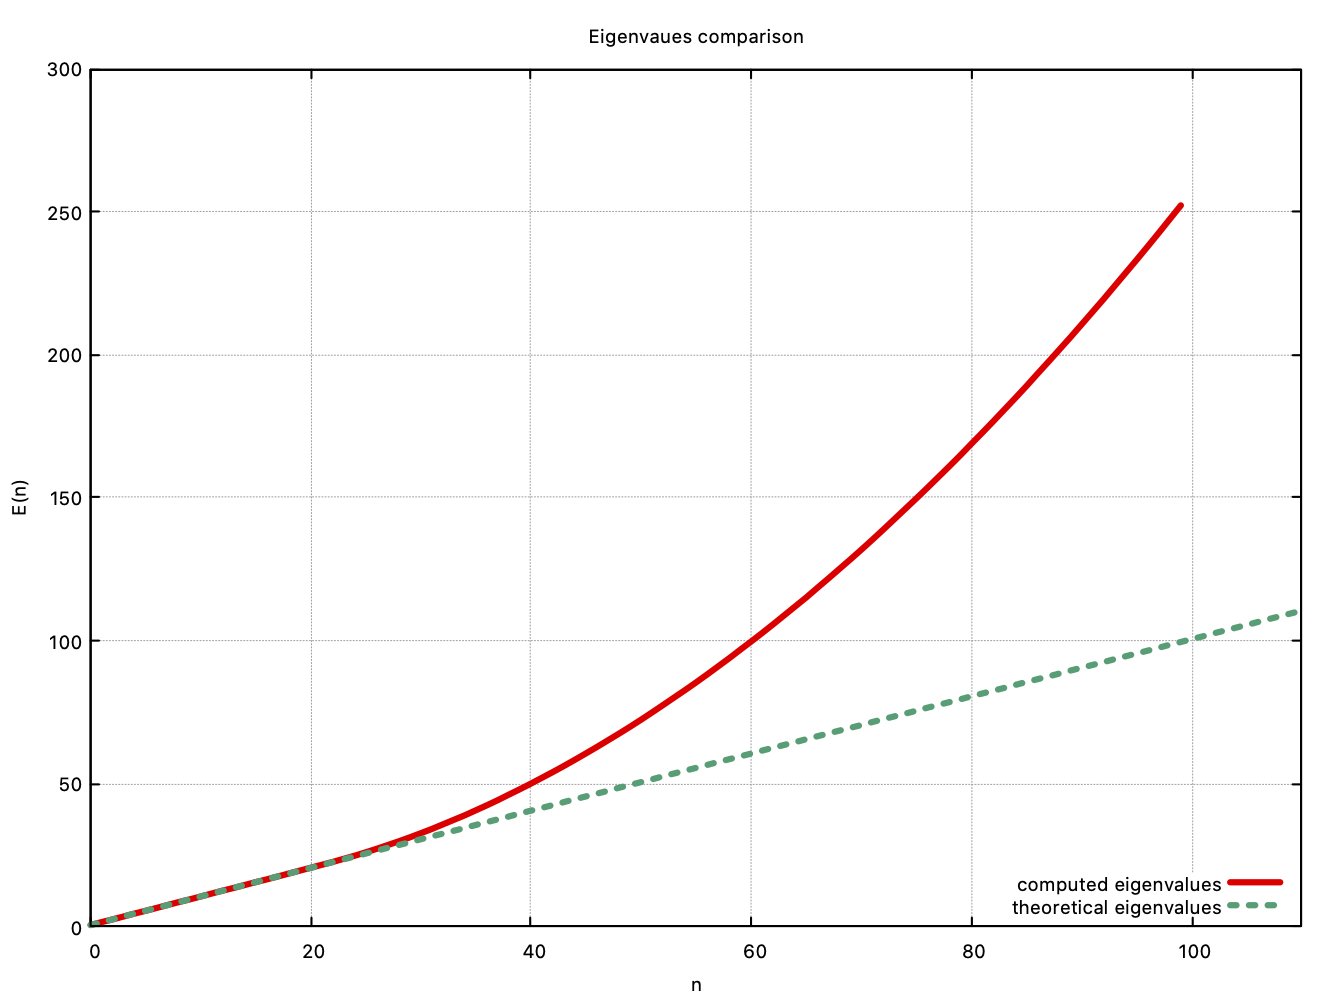
\includegraphics[width=.50\textwidth]{eigenvalues_comparison}\hfill
\end{center}
In the figure above we can appreciate the eigenvalues comparison. We see that, due to discretization, the the computed eigenvalues begin to diverge from the theoretical ones pretty early, around the $25^{th}$ value.




\begin{figure}[h]
    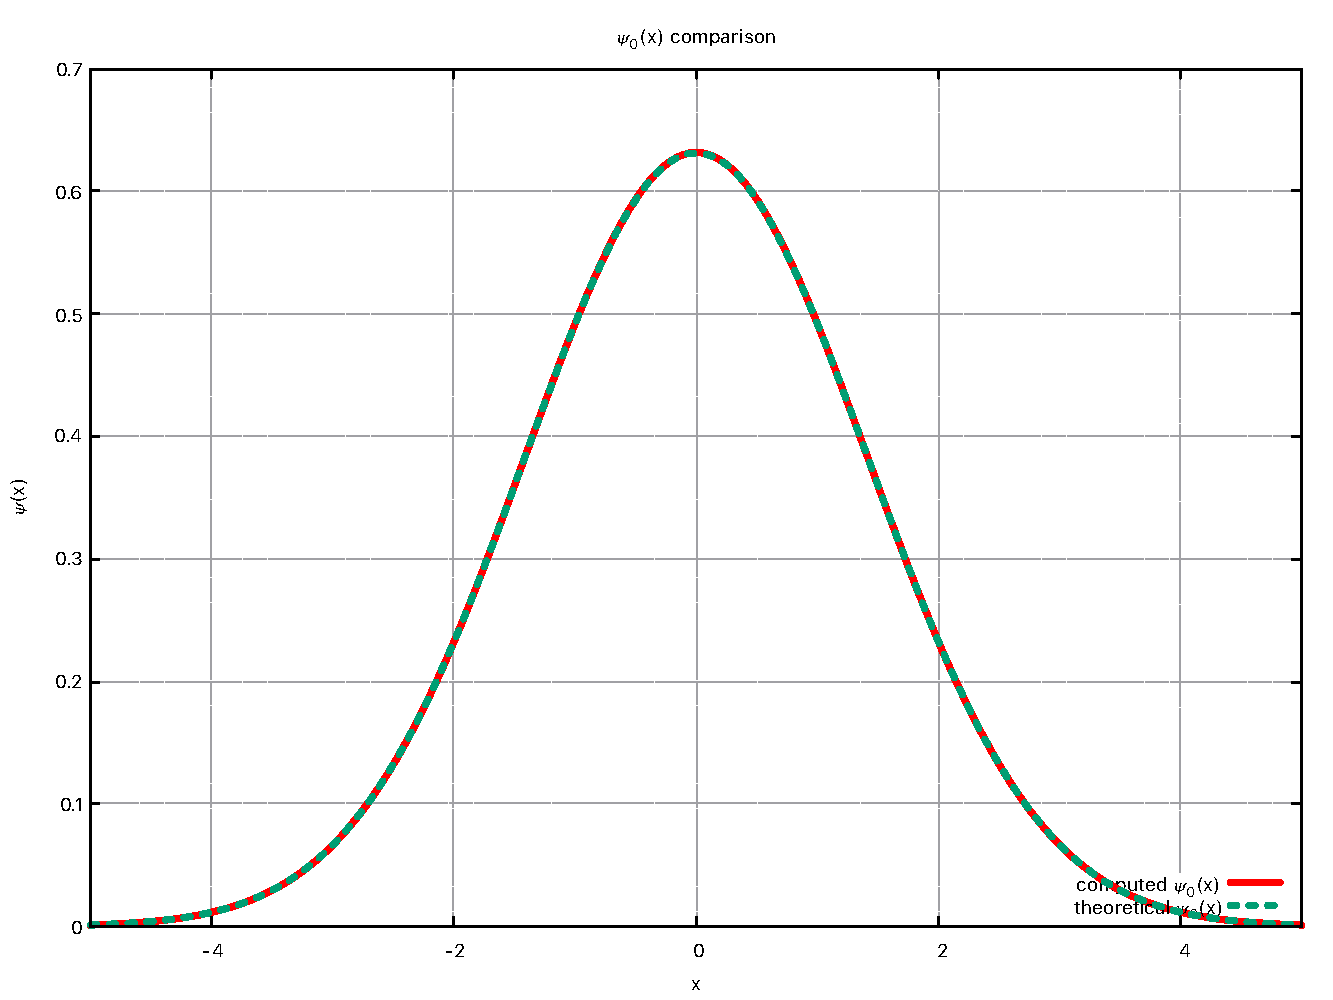
\includegraphics[width=.45\textwidth]{psi_0}\hfill
    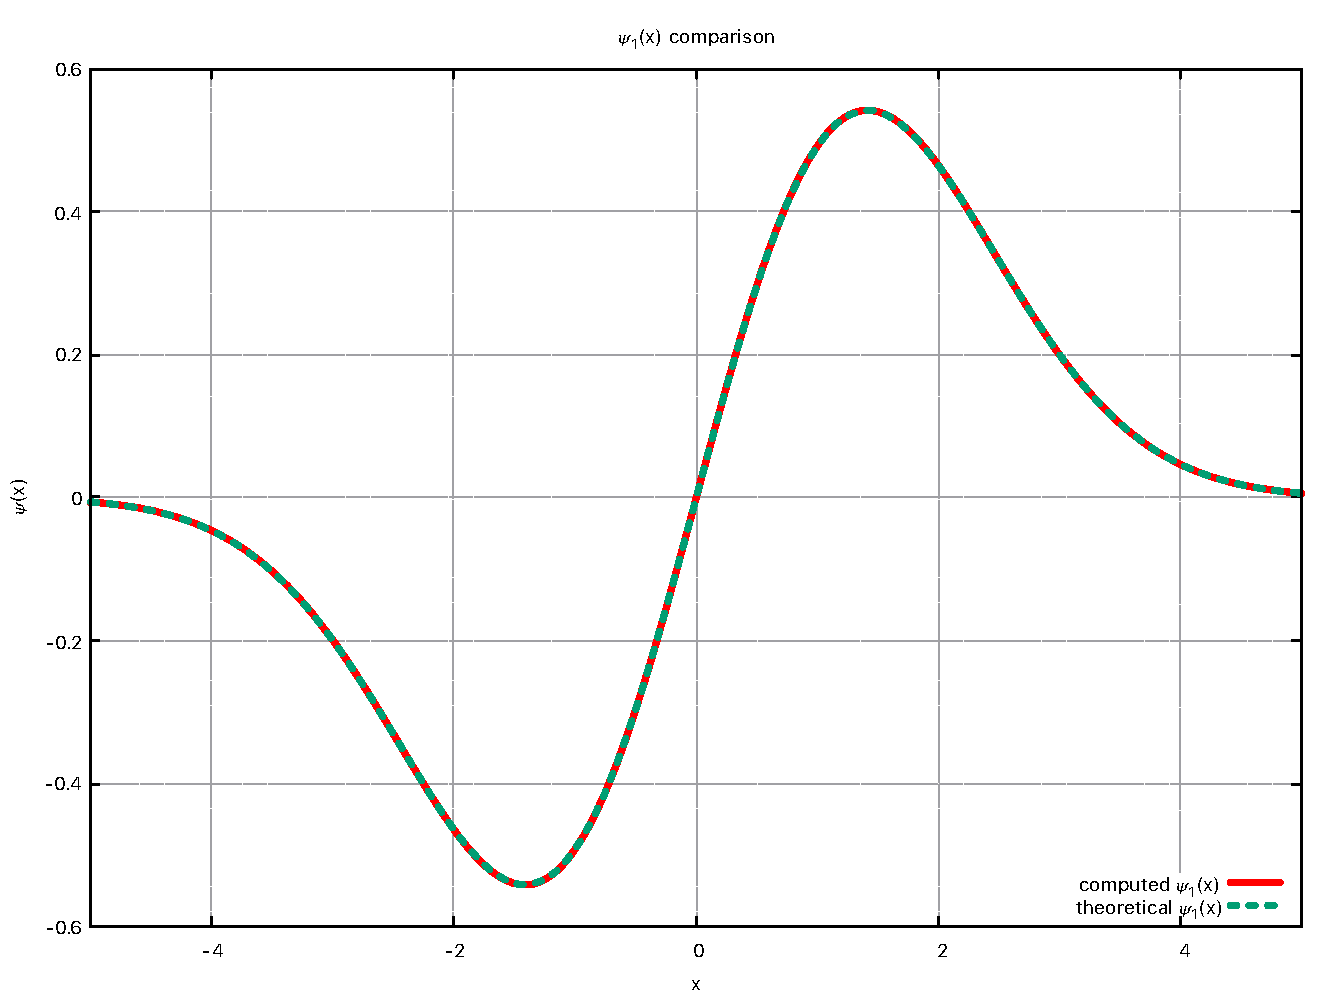
\includegraphics[width=.45\textwidth]{psi_1}\hfill
    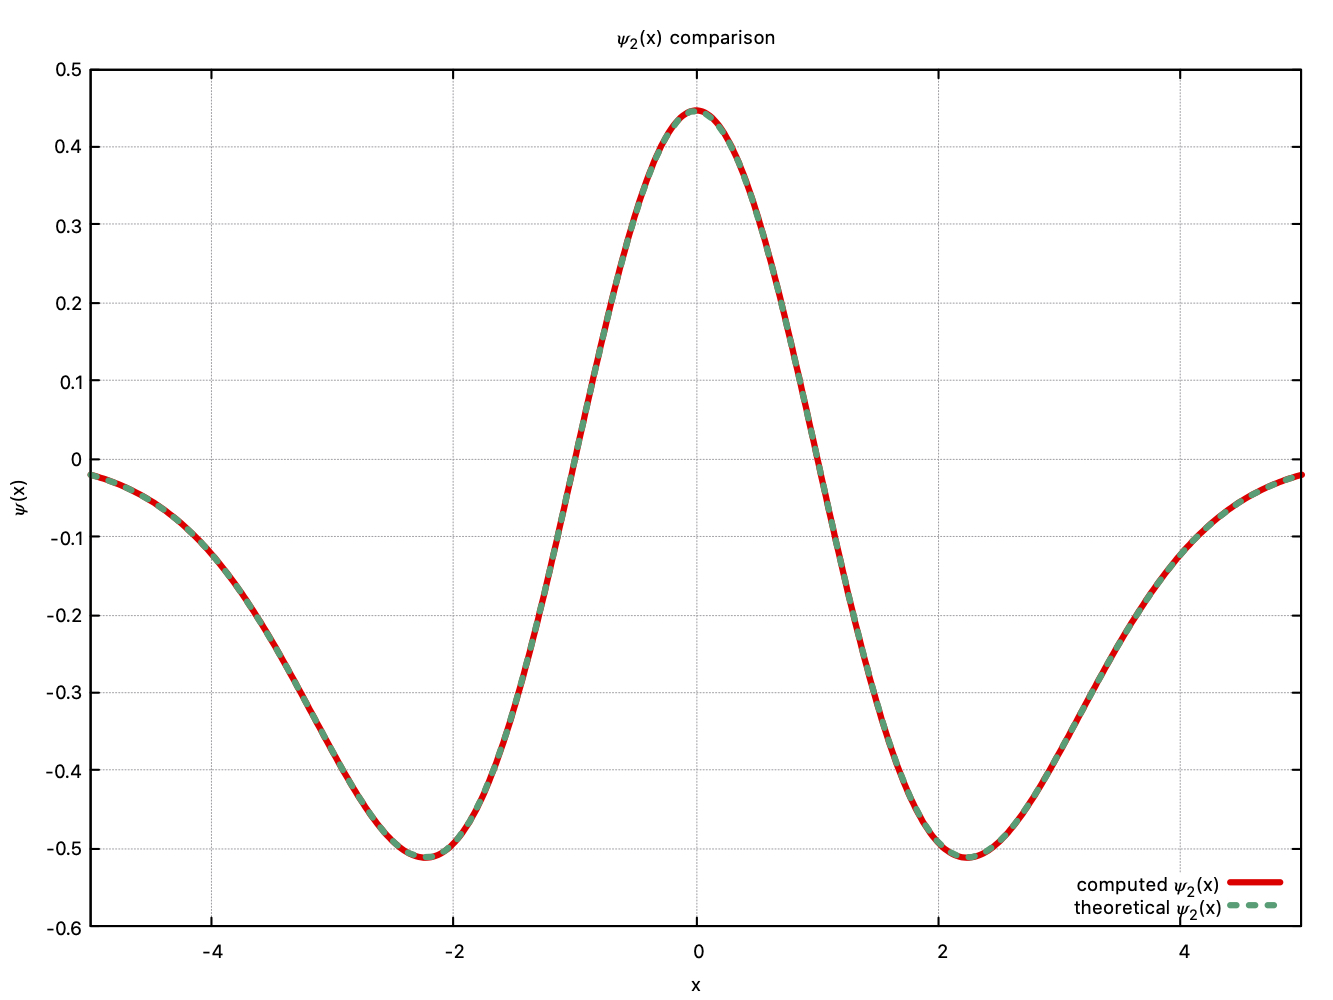
\includegraphics[width=.45\textwidth]{psi_2}
%    \\[\smallskipamount]
%    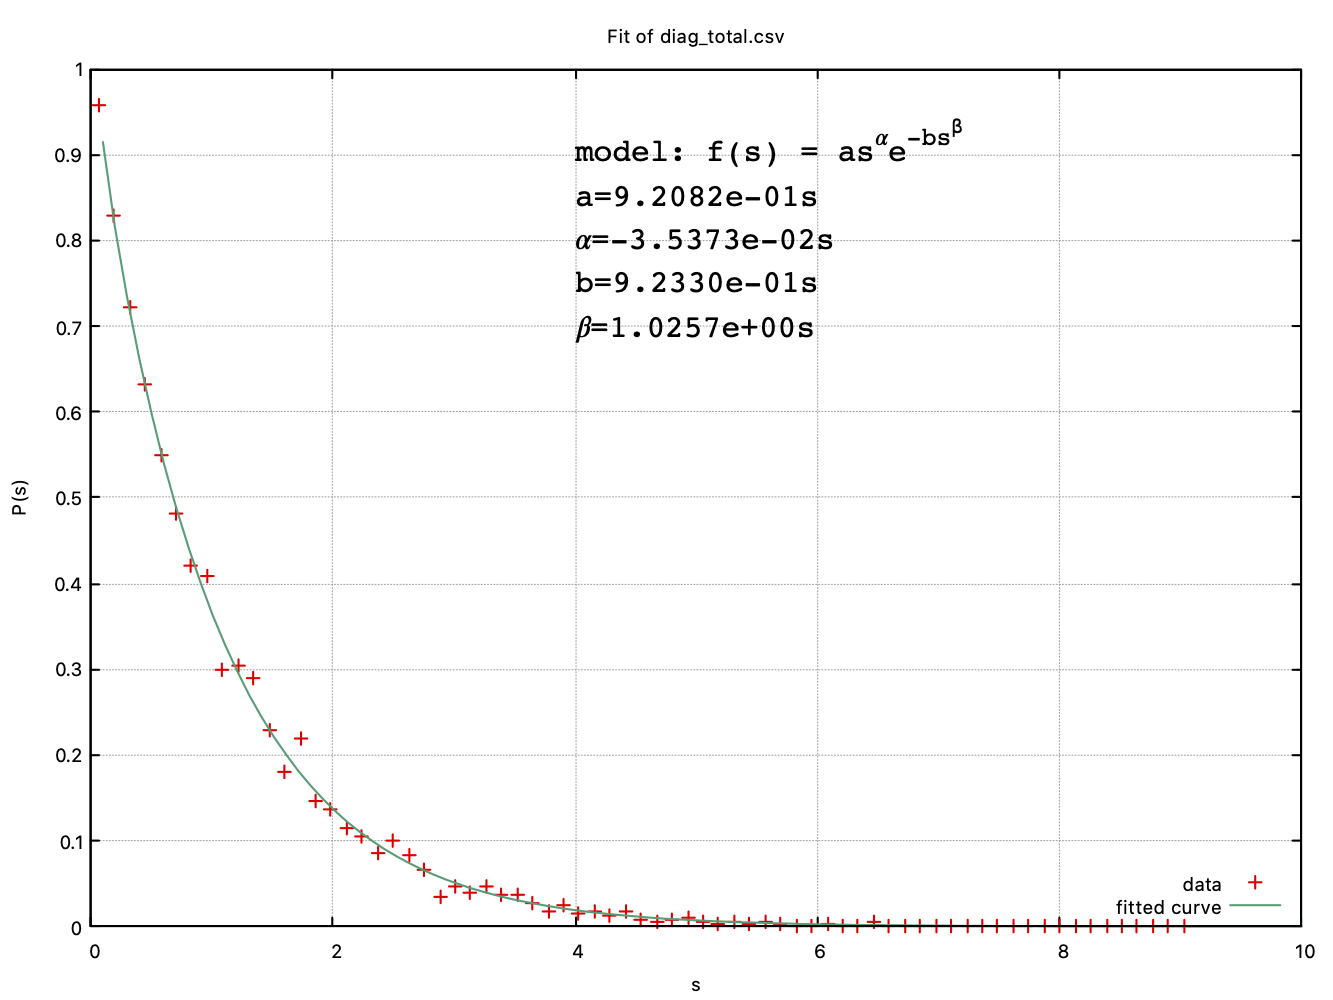
\includegraphics[width=.33\textwidth]{diag_total}\hfill
%    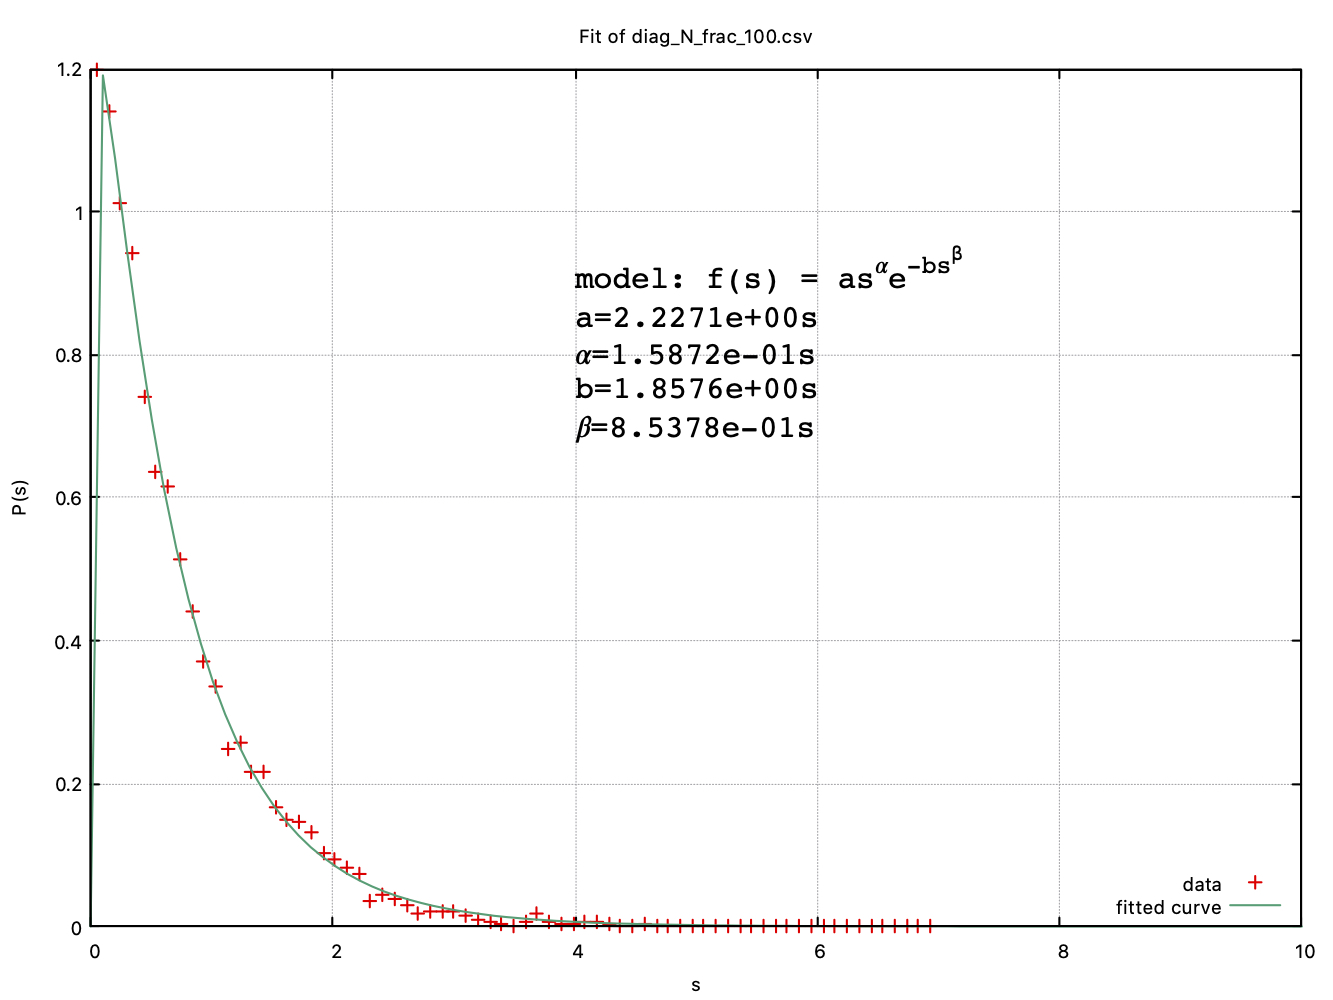
\includegraphics[width=.33\textwidth]{diag_N_frac_100}\hfill
%    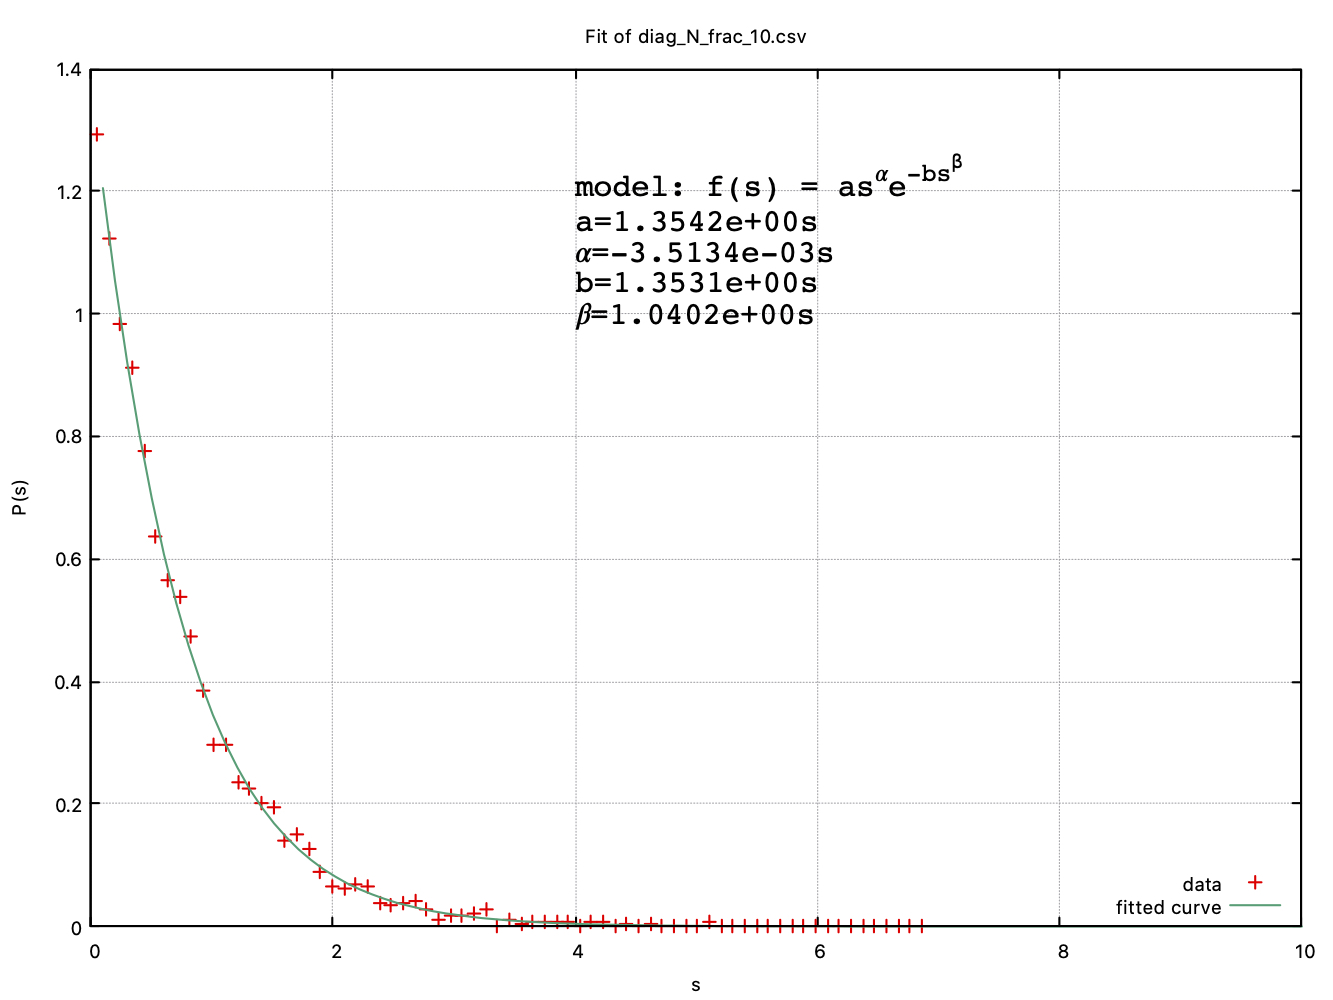
\includegraphics[width=.33\textwidth]{diag_N_frac_10}
    \caption{The comparison between the first three theoretical eigenfunctions and the computed ones}\label{fig:foobar}
\end{figure}

\section{Self-evaluation}
I think the main objectives of the exercises are reached. About the correctness of the code, I implemented several tests during the developing phase and the results are pretty good. The discrepancy between the computed eigenvalues and the theoretical ones is due to the discretization of the problem and the approximation of an infinite matrix with a finite one.

For what concern the numerical stability of the program, we face two major challenge from this point of view: the division of the elements of the matrix for the small value $h$, and the normalization of them after the diagonalization process. The program seems to have no problem from this point of view. Another issue could be the choice of the interval in which solving the problem, this has been choosen by look.

The chosen discretization (1000 points in an interval with boundaries of the order of 100) is sufficiently accurate to obtain successfully the eigen- functions, as we can see from the figures.

For what concern the flexibility I implemented all the routines used in the program in a module in order to have the possibility to reuse them in future works.



\end{document}
